\chapter{Introduction}
\pagenumbering{arabic}

\epigraph{Everyone in a complex system has a slightly different interpretation. The more interpretations we gather, the easier it becomes to gain a sense of the whole.}{Margaret J. Wheatley}


%% - Emerging of Information technology 
How is it possible for the nail size chip in our phone to understand us speaking or to recognize our face among thousands of people? 
It seems like magic that comes from science fiction and in less than a decade has become a contingent reality: every image of all phones is automatically tagged, every face recognized and all conversations typed.
It is not a very surprising fact though that, as a result, many people are actually rising concerns about this growth of technology and even governments are tightening regulations to guarantee the privacy rights against the economic use of people personal information.
%
%% - We can profit of IT for scientific experiment
Nonetheless, beside this new information business, those novel solutions that are mainly pushed by private interests are also very commonly released with open-source licences, thus being available to the scientific community. The idea is that vendors take advantage from a good code quality and the proliferation of new ideas within the wide pool of open-source developers, and at the same time the community gets access to a cheaper hardware and very powerful software tools that can be adapted to any specific need.
%
%% - Data over algorithm -> ML over AI
This new era, led by information theory, is revealing not to emerge from complicate mathematical models but from the data themselves, joined with lower cost per computational operation in terms of energy consumption and components price. %TODO: sistemare %
The predominant role of data is on one side promoting the big infrastructures where huge amount of signals must be collated by efficient databases and promptly passed through analysis algorithms, on the other side it stresses the need of an efficient design of hardware that must be able to adapt to the changes in algorithms and data dimensionality. This transition from single process to big-data analysis matches the shifting interest from the general \ac{AI} approach to the \ac{ML}\footnote{Machine learning is a subset of \acs{AI}. As from the definition by Tom Mitchell, author of the book "Machine Learning": A computer program is said to learn from \textit{experience} $E$ with respect to some class of \textit{tasks} $T$ and \textit{performance} measure $P$ if its performance at \textit{tasks} in $T$, as measured by $P$, improves with experience $E$.}, while from the algorithmic perspective it established the preeminent role of \ac{ANN}.

%% - Experiments may use hard correlated signals
The classical scientific approach is to make hypotheses on an evidence insulating repeatable experimental values and to provide a model able to reproduce those values. But it is not uncommon that within a complex experiment many different systems coexist, each with its own representation model, exposing a non trivial connection with each others. There is also the intuitive perception that gathering more and more information about a phenomenon gives a more accurate representation, but this requires to manage all the possible non-linear correlations coming from the different nature of signals.
~
%% - NN universal approximation
On the other hand it can be proved that any continuous convex function of n-dimensional input variables can be effectively approximated with a n+1 width neural network~\cite{csaji2001approximation}\cite{hanin2017universal}.
%TODO: ESPANDERE %
~
%% - deep learning
The actual turning point in ML happened with the NIPS'12 publishing of AlexNet~\cite{NIPS2012_4824}, a massive GPU trained network that won the ImageNet Large Scale Visual Recognition Challenge\footnote{The ILSVRC (\url{http://www.image-net.org/challenges/LSVRC/}) evaluates algorithms for object detection and image classification at large scale. One high level motivation is to allow researchers to compare progress in detection across a wider variety of objects, taking advantage of the quite expensive labeling effort.} achieving a top-5 error 10.8\% lower than the runner up. 
The original paper's primary result was that the depth of the model was essential for its high performance, opening the era of Deep Learning~\cite{Goodfellow-et-al-2016}.

%% - this thesis data integration using deep learning
A complex and heterogeneous experimental system could then benefit of this methodology in many ways: the possibility to integrate many different kinds of signals, the robustness to react on missing or corrupted data in case a portion of the sensory system fails, and the flexibility to adapt to changes on both the parameters or the environment variables of the experiment.
%
This thesis dissertation will present a set of tools that exploit such data integration, using the deep learning techniques from both the hardware and software perspective, applied to a possible scenario of controlling the magnetic confinement of a nuclear fusion plasma. 
% TODO: add.. in addition we will present the hardware implementation suitable to achieve the task
%
%% this is indeed a complex experimental setup applied to RFX-mod
This is, indeed, a very complex task other than one of the main challenges of this century. In this context the \textit{RFX~consortium} is hosting RFX-mod, one of the most controllable fusion experiments currently active in fusion research~\cite{SONATO2003161}\cite{doi:10.1063/1.4806765}.
Recently a further update to the experiment (RFX-mod2) has begun, aiming to improve the responsiveness of the machine, together with the renew of the sensory system. The research application described in the present work fits in this environment with a specific design proposal that integrates a \ac{ML} based control loop to the overall chain of data acquisition and control.

%TODO: REVIEW DOPO AVER SCRITTO INTRO%
In the next section a brief introduction to the problem of magnetic confinement will be presented followed by a description of the intuitive principles that justify the application of this kind of control.




\section{Magnetic confined nuclear fusion}
% FUSION %
The referred nuclear process is the exothermic reaction that happens between two light atom nuclei that fuse together. A fusion process that produces a transmutation to a new nucleus lighter than iron-56 or nickel-62 generally yields a release of energy. These elements have the smallest mass per nucleon and the largest binding energy; so the fusion of light nuclei toward, as well as fission of elements beyond these elements releases the energy retained, resulting in a exothermic reaction.  This means that, with the purpose of extracting energy, the lighter elements (hydrogen and helium) are in general more likely to be the fusible fuel, while the heavier elements (uranium, thorium and plutonium) are more likely to be the fissionable one. 
Figure~\ref{fig:binding} shows the binding energy per nucleon as a function of the atomic mass number. The exceptional situation of 4 (He) is shown. Fusion processes ending in He show the largest exothermal response; the burning of 1 (H) to 4 (He) releases most of the energy available to fusion. The maximum of the binding energy is with 56 (Fe).
\begin{figure}[ht!]
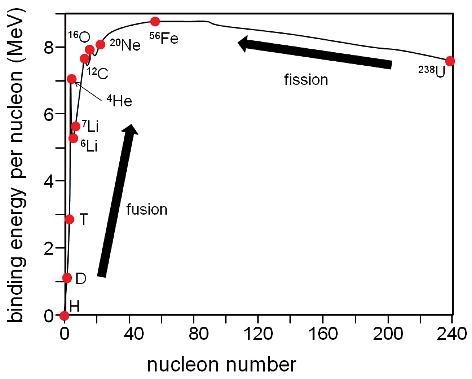
\includegraphics[height=0.25\textwidth]{img/binding_energy.jpg} \centering
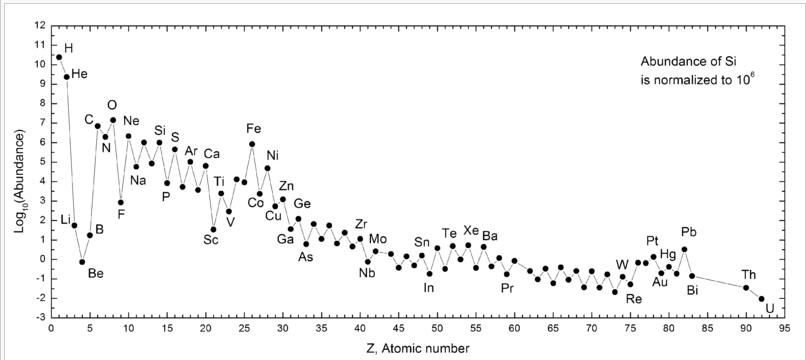
\includegraphics[height=0.25\textwidth]{img/abundance.png} \centering
\caption{Binding energy per nucleon for each element atomic number. }
\label{fig:binding}
\end{figure}

% FUELS and abundancy of elements %
The universe as forged by the Big-Bang was initially mainly formed by leptons along with simple elements: protons, deuterons, and a little quantity of helium and lithium. All the remaining set of the 92 known elements, from carbon up to uranium are afterwards the expression of the self-organisation of the universe - the formation of galaxies where the stars burn hydrogen as breeder material for new elements - enforced by gravity\footnote{ Lithium, Beryllium and Boron are relatively rare in cosmos since they had little time to form in the first expansion and are not directly synthesized by stars; their nuclei are actually destroyed within the star's core, however a small quantity can be produced by break-up of heavier elements in interstellar dust, as a result of impact by cosmic rays\cite{LiBeB_syntesis}}.

% Fusion and Fission in cosmos %
The production of heavy fission fuels by nucleosynthesis is generally ascribed to extreme astrophysical events like supernovas, that are able to reach enough energy to fuse nuclei into elements heavier than iron; when we use nuclear power coming from fission process we are indirectly recovering energy from those relatively rare events.
% 
On the other hand, as stated, the most common spread process in the universe is the burning of Hydrogen in the so called \textit{pp} chain reaction, firstly described by H.Bethe in 1939. 
In the core of a star, gravity produces high density and high temperature. The gas density in the core of our sun is 160 g/cm3, much higher than the densest metal, and the temperature is about $15\times10^6K$ ( $\simeq 1.5 KeV$ ). Under these extreme conditions the kinetic energy of particles and the continuous collisions disentangle all the electrons from the nuclei so the matter appears in the form of plasma. Protons (H-1) react with other protons to make deuterium nuclei (H-2) and positrons. The deuterium nuclei can merge to form a helium nuclei (He-4), or they can interact with other protons to make another isotope of helium (He-3). Two He-3 nuclei can fuse to make a nucleus of an unstable beryllium nucleus (Be-6) that breaks apart to give He-4 and two protons. Energy is released at each step.

In this sense the Hydrogen fusion is the most common way to obtain energy in the cosmos, and it is not by chance that the majority of the earth available energy resources are actually coming from the sun.

% Fusion in earth %
Starting from the Oliphant, Harteck and Rutherford experiments, that in 1934 provided for the first time the proof of transmutation accelerating Hydrogen~\cite{1934RSPSA.144..692O}, the attention quickly moved toward the plasma physics research by means of thermal excitation with the design of the \textit{tokamak} as a magnetic confinement device by the soviet physicists Igor Tamm and Andrei Sakharnov in 1950.%~\cite{}. 
%
% Cross section
% RR 
The fusion process between positively charged nuclei has to overcome the Coulomb repulsion, and the potential energy at a distance of a proton diameter is about 0.6 MeV. Nature eases fusion because the particles (the protons in this case) in this interaction adopt the characteristics of a wave, which allows them to leak into the energetically prohibited zone and to finally tunnel through the Coulomb barrier into the deep bound states of the newly formed nuclei. The potential energy at the distance of the de~Broglie wave length is about two orders of magnitude lower than the one within the range of the nuclear forces. The fusion yield depends on the density of the particles, their relative velocity and the nuclear interaction in the form of the fusion cross-section. 
The interaction processes are Coulomb collisions between charged particles. As the Coulomb collision rate is large compared to the fusion rate, the proton assembly (as well as the one of the electrons) can be described by a Maxwellian distribution. The governing kinetic parameter is the temperature rather than the individual particle energy in the assembly interactions scattering and fusion. This is the reason why we are speaking of controlled thermo-nuclear fusion.

% Lawson and why tokamak
The idea follows the simple principle that we need to produce fusion events at a rate that the system can, at least, virtually self sustain the reaction. 
\cite{Wagner.Friedrich:magnetic.confinement.intro}
The rate of fusion power normalized by the amount of external power needed is typically defined as the \textbf{Q} factor; 
% cross section rates and selection of thermal reaction
The selection of the proper reaction is guided, however, by searching for the highest reaction rate providing the highest fusion yield. This condition is fulfilled by fusing deuterium $D=\isotope{2,H}^+$, the heavy isotope of hydrogen, with tritium $T=\isotope{3,H}^+$, the super-heavy one.
% give temperature profiles for breakeaven and ignition

%
% magnetic confinement and MHD
The magnetic confinement relates to the fact that in those working conditions of temperature and pressure the reactants are completely ionized and all the particles subjected to the Lorentz force.
%
In the post-war period, some researchers began to consider different ways to confine a plasma. George Paget Thomson of the Imperial College London proposed a system now known as z-pinch, which flows a current through the plasma. Because of the Lorentz force, this current creates a magnetic field that draws the plasma on itself, keeping it away from the walls of the reactor. This eliminates the need for magnets on the outside, avoiding the problem noticed by Fermi. Several teams in the UK built a series of small experimental devices using this technique in the late 1940s.
%
%% LINEAR (CYL) CONFIGURATION
%
% - theta pinch can not be bent in a torus.
% Theta pinch equilibrium is easy to find ... see MHD
%
% - solution is the z-pinch 
% the MHD equilibrium can be solved by the Bennet relation
% In contrast to the Θ-pinch, for a Z-pinch it is the tension force and not the magnetic pressure gradient that provides radial confinement of the plasma
% it is not stable but can be bent in a torus
%
% screw pinch - general combination
% Though the momentum equation is non-linear, the Θ-pinch and Z-pinch forces add as a linear superposition, a consequence of the high degree of symmetry.
% the stability is granted by theta component and zeta brings the possibility to realize a toroidal shape.
%
%
Nowadays several families of magnetic configurations characterize different kinds of devices; the structural design of each fusion machine reflects the arrangement chosen for the internal field. the best topological configuration seems to be the torus. The main reason of this choice is due to the fact that the wanted pinch effect of the magnetic field is created by a current that flows thorough the plasma and can be closed in a loop by the toroidal configuration; also any loss of particles that a linear configuration would suffer is avoided. Besides the torus is the only compact connected domain where it is possible to define a continuous vector field without critical points. In this situation lines are usually winded around the shape with helical paths. 
%
% In a magnetic field charged particles move in a helix  F = q · v × B.  q is the charge, v the individual particle velocity, B the magnetic field. In the direction perpendicular to the field, the excursion of the particle is limited to the Larmor radius $\rho_L$ . Because of the specific form of the Lorentz force as vector product of velocity and field, the particle momentum parallel to the field is not changed. Therefore, in a homogeneous field, magnetic confinement is insufficient because it applies to the perpendicular velocity component only. One has to involve and to accept systems with field inhomogeneity to improve confinement. Magnetic confinement systems differ in the way they cope with the confinement parallel to the field thus defining classes of confinement systems.
%
% In linear devices — the first confinement class — parallel confinement is improved utilizing the mirror effect. The basis of the mirror effect is the magnetic moment μ = 12 mv ⊥ /B of a magnetised charged particle, which is a constant of motion.
% An electron or ion, which is thermally agitated with velocity v = (v ⊥ , v  ) and which moves
% from a zone of low field B min into one with higher field increases its perpendicular
% velocity v ⊥ as a consequence of μ = const. On the other hand, the kinetic energy of the
% plasma species is also a constant of motion with the corollary that the parallel velocity
% v  decreases. If the field is sufficiently large v  → 0. At this field, the mirror field B max ,
% the particle comes to a full stop. Thereafter, it is accelerated back to the low-field
% zone by the force −μ · grad  B. If the field system is built in a symmetric way, the
% game repeats itself at the other side with the outcome that the mirror effect causes the
% particles to bounce between two mirror points and to stay in the neighbourhood of the
% field minimum thus improving confinement. In an actual mirror machine, characterized
% by B min and B max , two classes of particles, discriminated by v  /v, have to be considered.
% If this velocity ratio is small, a particle is reflected by the magnetic mirrors as described
% above and represents a trapped one. Otherwise, it is slowed down along its trajectory
% toward higher field but does not reach the point with v  /v = 0. These particles escape
% the mirror. The boundary is given by v ⊥
% /v 2 = B min /B max specifying a loss-cone in
% phase space spanned by v ⊥ and v  as coordinates.

% The confinement of simple mirror machines is insufficient because the transparency
% of the mirror is too large. Still, we continue describing the confinement situation of the
% mirror because the concepts help us to understand the physics of more relevant confine-
% ment systems. Up to now, we have ignored collisions between the plasma species. Of
% relevance are the collisions in phase space of the trapped particles occupying the low-field
% zone scattered into the empty loss cone. Because of their higher velocity, electrons are
% scattered more frequently into the loss cone than the ions. As a consequence, the plasma
% is polarised and charges up positively. The formation of an electric field keeps back
% the escaping electrons by electrostatic means and accelerates the ions. For a transport
% equilibrium, the so-called ambipolar electric field enforces flux equality Γ e = Γ i between
% the differently charged plasma species of different masses and different kinetic properties.
% A confinement concept avoiding mirror losses is toroidal confinement realised in a
% plasma ring as shown in fig. 4. In this case, the magnetic coils are arranged in a closed
% ring thus avoiding end-losses. This geometry defines the class of toroidal confinement
% systems. An unavoidable feature is the inhomogeneity of the toroidal field with a higher
% field closer to the vertical symmetry axis. The field gradient points to the symmetry axis.
% This field inhomogeneity leads to rather unpleasant consequences: The Larmor orbits of
% the charged particles are not closed causing drifts. Ions and electrons drift parallel to the
% symmetry axis and leave their magnetic field line. The drift of electrons and ions is in
% opposite direction leading to an additional vertical electric field. A second parasitic drift
% appears now in the crossed-field arrangement of vertical electric and toroidal magnetic
% field. Like in the Hall effect an E × B drift appears perpendicular to both E and B tor
% directions, which causes the plasma torus to expand radially. No force equilibrium is
% established.

% The saving idea was to introduce rotational transform. A second field component
% B pol is introduced with a perpendicular (poloidal) component. A field line with the
% components (B tor , B pol ) winds around the torus in a helix (see fig. 4) and does no longer
% stay in a plane rather maps out a toroidal surface. The vertical charge separation is
% avoided because the up-down sides of the torus are short-circuited by the helical field
% lines connecting these regions. Macroscopic radial equilibrium can be provided.
% The essence of magnetic confinement is the development of a nested system of toroids
% with field lines, which encircle the tori toroidally and poloidally and with a field line
% density, which is higher at the inside than the outside (torus effect). The nested toroids,
% called flux surfaces (see fig. 4), are magnetically isolated and not connected by a field
% line with a net radial component.
% The way the poloidal field component is produced defines confinement classes within
% toroidal systems. The simplest one is using the potential of a plasma to carry a current. A
% ring current flowing inside the plasma, the plasma current I p , produces the poloidal field
% component B pol . As the temperature of the electrons, defining the electrical conductivity
% of a plasma, is highest in the plasma core, the current density profile j(r) peaks there.
% Such systems are called tokamaks [7] and are a Russian invention of the ’50s of last
% century( 8 ). Figure 5 shows the principal set-up of a tokamak. The major attraction of
% the tokamak is that I p can be produced by a pulsed transformer whereas the plasma
% ring surrounding a central primary coil acts as secondary winding. In tokamaks, the
% ratio of B tor /B pol > 1. Another concept with plasma currents is the reversed field pinch
% (RFP) with B tor /B pol ∼ 1 [8]. Tokamaks and RFPs belong to the category of internal
% confinement systems because part of the confining magnetic field is produced by currents
% flowing inside the plasma. 

%An alternative way is to produce the poloidal field like the toroidal one — by external
% coils. In this case, the coils have to wind helically around the torus. The field composition
% reminds of a multipole arrangement with coils being first helically twisted and then bent
% into a torus. Depending on the current direction inside the helical coils — unipolar or
% bi-polar — we speak of heliotrons/torsatrons or of stellarators. Both belong to the class
% of helical systems. Stellarators are a US invention of the ’50s. Figure 6 shows a sketch
% of a classical l = 2 stellarator with helical coils. Helical systems belong to the category
% of external confinement.
% Toroidal systems share common descriptors. In the simplest case with circular poloidal
% cross-section the torus geometry is defined by major radius R and minor radius a (see
% fig. 4). The ratio A = R/a is called aspect ratio. The rotational transform ι of a flux
% surface is defined by the winding law of the field lines given by ι/2π = AB pol /B tor . RFPs
% have a larger ι than tokamaks. In case of helical systems, B pol is determined in a complex
% form by the external helical coils system, which is described by the number of coils e.g.
% 3 heliotron coils with unidirectional current yielding an l = 3 heliotron. In this case the
% poloidal cross-section has the shape of a triangle. In case of a stellarator with 4 helical
% coils and bi-polar currents, we have 2 pairs of coils and an l = 2 stellarator (see fig. 6).
% Its poloidal cross-section is elliptical. Another important stellarator descriptor is the coil
% pitch. The coil winding laws are such that the coils ultimately close. The field pattern
% of helical systems is periodic in toroidal direction. The toroidal periods can be m = 5
% (Wendelstein 7-A, Germany [3]) or in case of tight windings e.g. m = 10 (Large Helical
% Device, LHD, Japan [3]).
% Simple tokamaks have a circular cross-section. Equilibria at higher plasma currents
% are possible when the cross-section is elongated or even has triangular shape. Modern
% tokamaks benefit from the higher current:


\section{Magnetic confined plasma experiments}

Among the several proposed solutions for thermonuclear confinements devices, the torus appeared as the most topological advantageous. Torus is the only compact manifold connected and orientable where it is possible to define a continuous vector field without critical points\footnote{once a vector field has been defined on the surface of the torus, there are no points where it reaches zero; this characteristic let the field lines to reconnect on themselves minimizing the energy spent and maximizing the stability of the plasma}.
In this case the field configurations consist on a set of magnetic toroidal and poloidal components. In \Figure{\ref{fig:intro_toroidal_coords}} a toroidal coordinates ($r,\theta,\varphi$) reference system is represented, where:
\begin{figure}[h!]
    \centering
    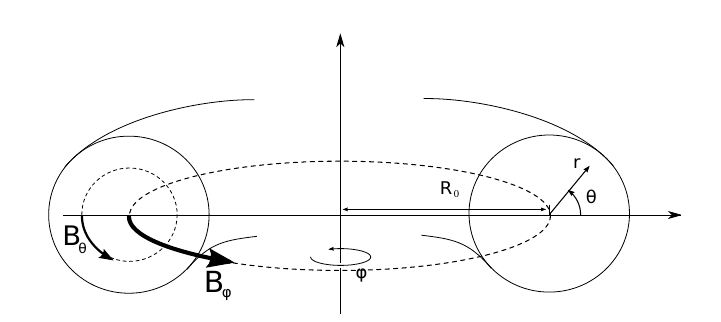
\includegraphics[width=8cm]{img/1_intro/toroidal_coords.png}
    \caption{Toroidal coordinates reference system}
    \label{fig:intro_toroidal_coords}
\end{figure}
\begin{itemize}
    \item $r = $ radial distance from central circular axis,
    \item $\vartheta = $ poloidal angle,
    \item $\varphi = $ toroidal angle.
\end{itemize}
Depending on their characteristics, the magnetic confined machines are divided in three principal categories:
\begin{itemize}
    \item \textit{Tokamak}, where both the toroidal and poloidal field components are present but with a net toroidal predominance that assumes essentially stabilization functions.
    \item \textit{RFP}, where the toroidal component is almost comparable to the poloidal to the extent that it reaches an inverted value at the boundary ( hence the name "\textit{reversed} field pinch"). Compared to the Tokamak configuration the stability of plasma is much more critical, but higher in efficiency.
    \item \textit{Stellarator}, where the geometry of the field is built by a complex displacement of non planar coils that encourage the winding of the plasma column.
\end{itemize}

\subsubsection{Tokamak configuration}
In the \textit{Tokamak} systems the toroidal field $B_\varphi$ is produced by a toroidal solenoid winded around the vacuum chamber, while the poloidal field $B_\vartheta$ is created by a strong toroidal current $I_p$ that flaws within the plasma. This current is in turn induced by means of solenoids coupled by the plasma ring (sometimes concatenated with a central coil). The same current is also used to heat the plasma by Joule effect ( Ohmic heating ) with a specific power of $P = \eta J^2$, defined $\eta$ as the plasma resistivity.
%
A fundamental parameter to define the \textit{Tokamak} typical features is $\beta$ defined as:
\begin{equation}
    \beta = \frac{<p>}{ \frac{B(a)^2}{2\mu_0} }
    \label{eq:magnetic_beta}
\end{equation}
with $<p>$ the average value of plasma pressure within a poloidal section. This parameter is the ratio between the mean kinetic pressure exerted by plasma, and the magnetic pressure of the field that is needed to confine it; the value assumed by $\beta$ is thus the measure of how effective the magnetic configuration results when seen as an energy balance.
If we compute the \eqref{eq:magnetic_beta} using the typical $B_\varphi$ and $B_\vartheta$ values that are present in a \textit{tokamak}, the resulting $\beta$ is about $2-3\%$; this means that the most of the spent energy that \textit{Tokamak} uses is not for the confinement but is is almost all used to stabilize perturbations.
Another key factor that defines the relative intensities of magnetic configuration is the so called "\textit{safety factor}" $q$:
\begin{equation}
    q(r) = \frac{rB_\varphi(r)}{R_0B_\vartheta(r)}
\end{equation}
As it will be widely described in the following sections, the radial profile of this parameter has a fundamental impact on the overall stability of the plasma: in more detail, a stable plasma configuration can be obtained by maintaining the $q(r)$ function strictly monotonic.
\begin{figure}
    \centering
    \subfigure[]{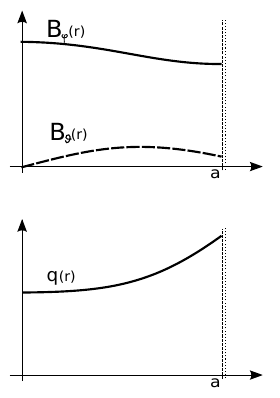
\includegraphics[height=5cm]{img/1_intro/tokamak_profiles.png} \label{fig:intro_safety_factor_profiles_a}}
    \subfigure[]{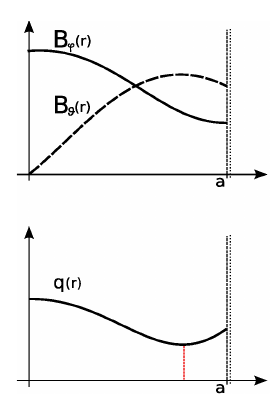
\includegraphics[height=5cm]{img/1_intro/rfp_profiles_norev.png} \label{fig:intro_safety_factor_profiles_b}}
    \subfigure[]{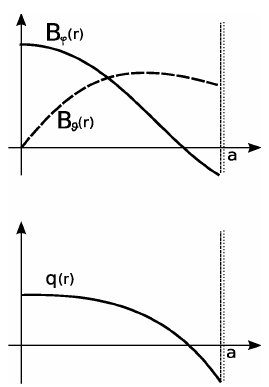
\includegraphics[height=5cm]{img/1_intro/rfp_profiles_rev.png} \label{fig:intro_safety_factor_profiles_c}}
    \caption{Magnetic field profiles for $B_\varphi$ and $B_\vartheta$, from the toroidal axis to the chamber boundary, for the toroidal confinement devices in \textit{Tokamak} configuration (a), \textit{RFP} without reversal (b), and \textit{RFP} with reversal (c)    }
    \label{fig:intro_safety_factor_profiles}
\end{figure}
As shown in \Figure{\ref{fig:intro_safety_factor_profiles_a}}, in the case of the \textit{Tokamak} configuration the monotonic property of the safety factor is guaranteed by an high ratio of $B_\varphi/B_\vartheta$. Still, because the poloidal fields is generated by the plasma current, to have such a high ratio of the fields it is necessary to maintain it under a certain threshold. This condition implies in effect a limitation for the possible Ohmic heating, bringing with it the need to find other means of additional heating, such as neutral particles injections (NBI), radio-frequency emissions resonating with cyclotron frequencies of electrons or ions, and so on.

\subsubsection{RFP configuration}
The \ac{RFP} is an axial-symmetric configuration provided with a toroidal current, similar to the \textit{Tokamak}. The difference between the two is in the ratio of the magnetic field components: while for the \textit{Tokamak} the toroidal field is of one order of magnitude over the poloidal, for the \textit{RFP} the two components are almost the same in average, and in the outer region the poloidal one tends to dominate. As a result, the most part of the magnetic field is generated from the plasma current itself, and with the same plasma current the total magnetic field that is exploited by \acs{RFP} is much lower that the one used by a \textit{Tokmak}. It can be also seen that, in the right conditions, once the plasma current has been induced, the toroidal field at the boundary inverts direction; this reversal gives a chance to obtain a monotonic factor $q(r)$ even with such low magnetic profiles. This is generally facilitated inverting the current direction on the coils of the toroidal system some instants after the pulse begins. For the \acs{RFP} model the profiles of $B_\varphi$(r), $B_\vartheta(r)$ and $q(r)$ are reported in \Figure{\ref{fig:intro_safety_factor_profiles_b}} and \Figure{\ref{fig:intro_safety_factor_profiles_c}} in the pre-reversal and reversal conditions.

Together with this reduced toroidal field intensity comes the possibility of reaching $\beta$ values much higher than those characterizing the \textit{Tokamak}. 
Given its magnetic topology, the RFP exploits the advantage of an easier technology involved in the electromagnetic system. This might be the case even for a reactor, where there might be no need for large superconducting magnetic coils; there is freedom in the choice of the aspect ratio and, in principle, ignition should be achievable with ohmic heating only.  
Although the high penalty payed by the \textit{RPF} is on the stability of perturbations that represents a profound limitation for the final achievable temperature, that remains one order of magnitude lower that the one promised by a \textit{Tokamak}.

% RW
A price to be paid for exploiting these advantages concerns magneto-hydrodynamic (MHD) stability. The safety factor q is in fact lower than 1 across the whole plasma, and negative at the edge. Figure 2(a) shows the q profiles of an RFP compared with those of tokamaks and stellarators. In the RFP q profile there are multiple resonant surfaces in the plasma, in particular for modes with poloidal mode numbers m = 0 and 1. This is shown in figure 2(b), which reports a typical RFP q profile. Two main kinds of global, current-driven MHD instabilities may be present in a RFP with resistive wall: (i) resistive kink/TMs, which are resonant in the plasma and are intrinsically linked to the sustainment of the configuration through the aforementioned self-organization process; (ii) RWMs, which are non-resonant ideal modes, slowed down by the resistive wall. RWMs in RFP are current driven and are present also at low plasma beta.


RFPs, however, can sustain very high plasma current and this makes it to be considered a potential fusion device with only Ohmic heating. On the other hand, the generation of plasma current needs a time variation of magnetic field which is sustained by the primary transformer. This time variation makes the devices, on some level, not in steady state. To overcome this problem, a toroidal configuration in which all the field components are generated by external coils is introduced. This device is the so-called stellarator. \Figure{\ref{fig:pinch_families}} shows a sketch of these two families. In the left graph, the red coils aligned toroidally are the toroidal field coils and the green helical ones are helical field coils. In the right graph, the red cylinder in the device center is the primary transformer. The red coils aligned toroidally are the toroidal field coils and the two green ones on the top and bottom of the device are the vertical stabilization coils. The stabilization coils are introduced because, due to the existence of Shafranov shift in toroidal devices, the plasma position needs to be optimized in order to avoid touches between the magnetic field and the first wall. 
The stellarator shows a much more complicated magnetic coil design than the one of the pinch family. Consequently, the manufacture process for magnetic coils are more complex for stellarators than for pinches. On the other hand, due to lack of plasma current, stellarators are almost free of disruptions.

Two dimensionless parameters are used to describe the RFP equilibrium. 
The pinch parameter \textbf{theta}, defined as:
\begin{equation}
    \Theta = \frac{B_\vartheta (a)}{ \left\langle B_\varphi \right\rangle }
\end{equation}
measuring how much the plasma and the magnetic field are pinched inside the torus; and the \textbf{reversal} parameter F, defined as:
\begin{equation}
    \mathrm{F} = \frac{B_\varphi(a)}{ \left\langle B_\varphi \right\rangle }
\end{equation}
that quantifies, instead, how much the toroidal field is \emph{reversed at the edge}.

The minimal model to compute the RFP equilibrium is the one-dimensional model governed by the MHD equilibrium equation $\nabla p = \Vec{j} \times \Vec{B}$ solved in cylindrical coordinates together with a parametric description of current and pressure profiles~\cite{Bonomo33}.
A more accurate model needs to add the toroidal geometry that produces outward radial displacement of magnetic flux surfaces, and hence a separation between the geometrical and the magnetic axis, i.e. the \textit{Grad-Shafranov shift}~\cite{freidberg2014ideal}. 
In this representation, RFP presents an axisymmetric equilibrium dependent on all toroidal coordinates $(r, \vartheta, \varphi)$  where the magnetic field lines are helixes. This RFP state (also called Single Helicity (SH) state that will be presented later on) can be described in terms of a helical Grad-Shafranov equation~\cite{Bonomo35, Bonomo36}, which represents the full 3D solution to the MHD equilibrium equation.


\section{RFX Experiment}
The first installations with $B_\varphi$ and $B_\vartheta$ fields of the same order of magnitude, i.e. the so called \textit{screw pinch} or stabilized \textit{zeta pinch}, started to operate at the beginning of the 60s; the most relevant was the ZETA\footnote{ZETA (Zero Energy Thermonuclear Assembly) that operated from 1954 to 1958 in Harwell (UK).}. At the time the results were considered mediocre: the machine presented a turbulent regime, followed by sporadic quiescent phases difficult to interpret. The first theoretical model was proposed by C.~B.~Taylor in 1974\cite{taylor}: He speculated, and proved afterwards, that the quiescent condition in ZETA corresponded to the spontaneous switch from the stabilized \textit{zeta pinch} system to the RFP by means of a self reversal of the toroidal field; and that this was also due to a minimum of the magnetic energy.

In the late 70s a research on such self phenomena started in Padova and brought to the making of RFX ( Reversed Field experiment ), a reversed field experiment machine with major radius $R_0 = 2m$ and minor radius $a = 0.5m$, that proved to be able to sustain a plasma current of $2MA$. In the period between 2001 and 2004 the same machine was modified to RFX-mod\footnote{in 1999 a severe damage of the plant was caused by a fire on the electrical source equipment. The experimental activity was not recovered until December 2004, after an intense rebuild of the plant and upgrade of the machine itself.} adding an active feedback control that widely improved its results.
\begin{figure}[ht!]
\centering
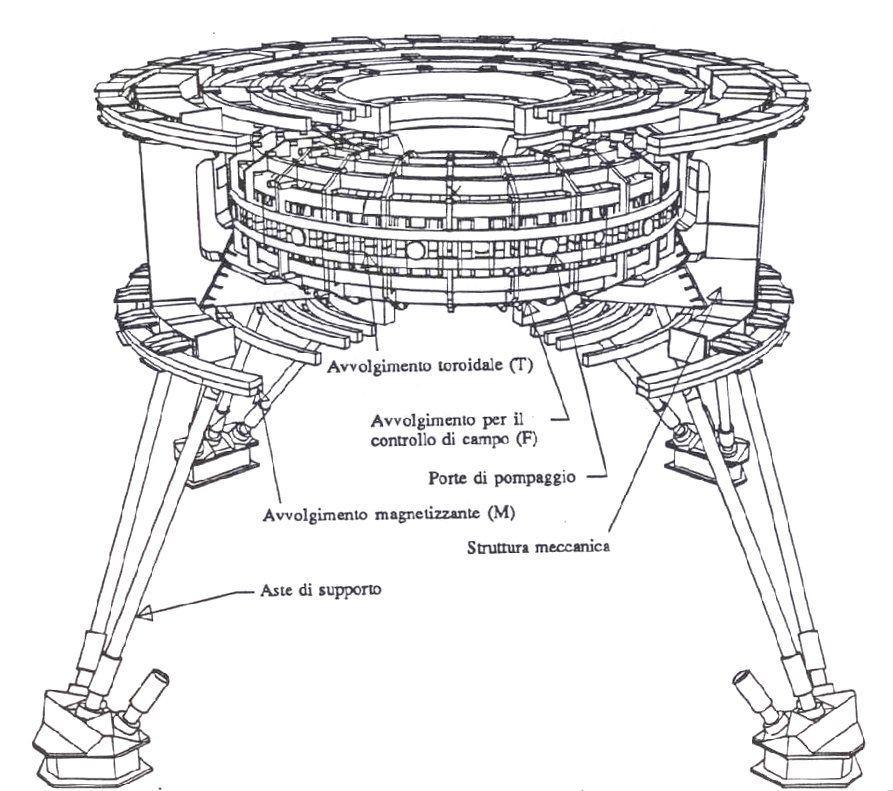
\includegraphics[width=0.5\textwidth]{img/rfx2}
\caption{ Perspective view of the RFX experiment }
\label{img:rfx}
\end{figure}
%
RFX is built of a vacuum vessel made of INCONEL~625\footnote{a nickel chromium molybdenum alloy that is frequently used to produce a stiff material with high temperature tolerance and good mechanical properties} and completely internally covered by 2016 carbon plates that shield it from sudden heat impulses generated by the plasma; it can resist to temperatures beyond 350C, and achieve ultra vacuum conditions $(P < 10^{-6} \text{mbar})$.
The structure, also called \textit{liner}, is composed by 72 cuneiform elements, shown in \Figure{\ref{fig:rfx_liner}} all displaced at 5 degrees one from the other in the toroidal direction, with an internal 1mm layer, an external 2mm, joint with a corrugated ring of 0.5~mm.
\begin{figure}[ht!]
\centering
\subfigure[]{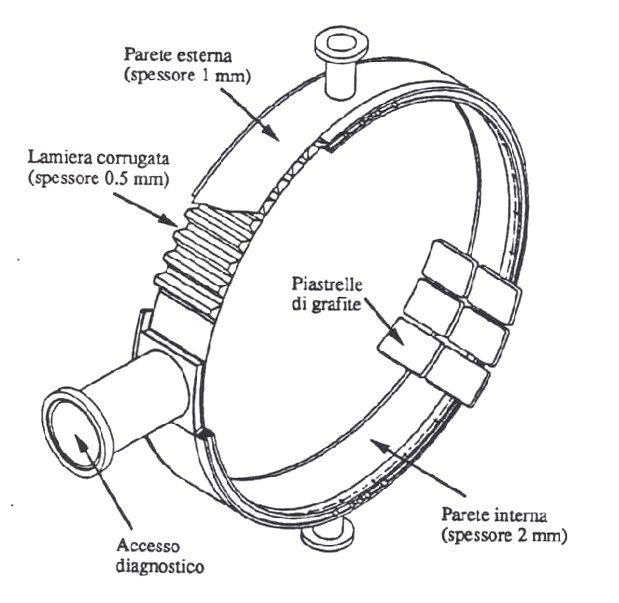
\includegraphics[width=0.4\textwidth]{img/rfx/liner_element.png} \label{fig:rfx_liner}}
\subfigure[]{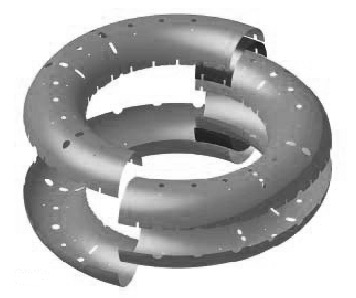
\includegraphics[width=0.4\textwidth]{img/rfx/shell.png} \label{fig:rfx_shell}}
\caption{ Perspective sketch of one of the 72 RFX vacuum chamber elements (a), RFX stabilizing shell components (b). }
\end{figure}


On the outer side the vacuum chamber is completely wrapped in a high conductive shell; the former choice was an aluminum foil, subsequently substituted by a chopper 3mm film in RFX-mod. The shell is composed by 4 parts of 180 degrees angular width on the poloidal direction, and a bit more on the toroidal one. Once the parts were assembled together, as shown in \Figure{\ref{fig:rfx_shell}}, two gaps remained unwelded: one on the toroidal direction and one in the poloidal direction in order to permit the magnetic fields to penetrate inside the shell\cite{th13}.

All currents, induced on the shell by radial field components (generated by a plasma perturbation), tend to counteract the plasma movement itself. This characteristic of the shell is able to stabilize fast perturbations\footnote{perturbations that happen in times in which the field remains stitched to the plasma (Alfv\'en theorem).} contributing to the horizontal equilibrium on the very initial states of the pulse~\cite{th19}. The value for a vertical field penetration time is about $\tau_w = 50 ms$\cite{th12}.


\section{Plasma control based on machine learning}

% supervised and unsupervised learning.
The very basic idea that defines the machine learning itself is to build a model that learns from experience. This happens it two ways: the model can be trained from a dataset that contains the true interpretation, or it can be trained without any information generating a representation of data itself. The two approaches are respectively called \textit{supervised} and \textit{unsupervised} learning.

Supervised learning is the task of learning to map input to output based on a set of previously known input-output pairs. It infers a function from labeled training data consisting of a set of training examples composed by pairs of input objects (typically vectors usually called features) and desired output values (called labels). The algorithm analyzes such data and produces an infer function, which can be then used for mapping new examples. In an optimal scenario this will allow to identify the class labels for unseen instances, because the learnt function will have generalized from training data to unseen situations.
The supervised learning are the most common and most used methods, because they provide a result with a direct meaning. 
This is well interpreted by neural networks that are actually one of the most simple approaches to machine learning, but at the same time one of the most promising, because they can very easily scale to tackle almost any kind of task with the same base units.
%
In principle the label information, i.e. the dataset ground truth that we use to "supervise" the model training, can be almost anything; we could choose to train a network to guess the whether forecast by counting the number of birds that fly by the yard. Any kind of data could be a useful argument if a weak relation could be extracted between data and labels.
From a statistical point of view, neural networks are nothing more than devices adapting to represent non-linear curves. 
Nevertheless, fitting a non linear curve is not a trivial task; the actual complexity of an interpolated model is of crucial importance. 
Indeed, while changing the complexity of the model, the best measure for the training data that the model can obtain becomes increasingly good, but the empirical fit performance first diminishes, then increases again. This happens because a model that is too complex starts to adapt to the training data and generalizes badly. In other words we could say that it learns how to represent the very training set, not any input data.
%
% course of dimensionality
The problem is the dimensionality of the input space. If the input feature vectors have very high dimension, the learning can be difficult even if the true function only depends on a small number of those features.  This is because the many "extra" dimensions tend to confuse the learning algorithm producing high variance on training. 
This problem is known in machine learning as the \textit{course of dimensionality}.
For this reason high dimensional inputs typically require the tuning of classifier to have low variance and high bias. In practice, if irrelevant features from the input data can be removed, this is likely to improve the accuracy of the learned function. 

A fusion experiment is very like to fall in this issue, because to acquire all the different aspects of the plasma characteristics a huge amount of diagnostics are required. A single kind of measure does not provide all the necessary information, and the actual glue that fixes the characterization of the machine has always been the physical model that subtends the phenomenon.
But this is not trivial as well: the data can be affected by many kind of noise and they may have only a partial access to the required variables that are needed for the physical model to run.

To solve this problem there are many algorithms for feature selection that seek to identify the relevant features and discard the irrelevant ones. 
Other methods require to apply preconditioning constraints that add existing relation among data: for instance, if we know that the data samples are ordered sequences, it makes sense to introduce algorithms that exploits this property such as the convolution.
This is an instance of the more general strategy of dimensionality reduction, that seeks to map the input data into a lower-dimensional space running the supervised learning algorithm or prior to it. 

A further possibility for the interpretation of high dimensional data could be their statistical representation.
This is the aim of the unsupervised learning, where similar algorithms are applied to feature without the aid of external information. The target this time is not to look for a given relation but for a representation of the data itself.
Several methods can be applied to achieve such dimensionality reduction: for example the principal component analysis, the singular values decomposition, and factor analysis among linear approaches; or the Autoencoders~\cite{Hinton504} as a neural network non-linear approach.

As stated, Autoencoders exploit the neural network architecture. They are built to have the same number of neurons both at the input and the output layers and the topology is organized to have an internal layer with less neurons to form a bottleneck. The training tries to match each data sample with the output by direct comparison.
The output values of the hidden smaller layer are then the reduced coordinates in the new space with a smaller dimension.
The overall path of the data through the network can be divided into two steps: a first net reduces the data dimensions \textit{encoding} the features in a small set of values, then a further net recovers the input data from the \textit{decoding} of the latent representation. 

Those values can be thought as the latent states of a non linear model representation and can be used to extract the new features that feed a supervised algorithm. In addition, a bayesian description of the latent variable can be applied, creating a true latent space. This is the case of the so called Variational Autoencoder (VAE) that is a \textit{generative} algorithm that recently gained a lot of attention.
In this case we create two distinct domains: the domain of the data and the latent one. On such models encoding a data can be seen as the inference to the latent space value, and decoding back to the data domain is referred as the \textit{generative} process. Hence the name of \textit{generative algorithms}.


% it is not the lose of the model
% - model can be applied to add information ( fourier for example )
% - model can be added to confront the dimensionality of the latent space

% no free launch theorem (perche neural networks)

% introduction to the bicycle example 
\subsubsection{How to ride the bicycle}

The primitive idea of the neural networks was originated by the first studies on brains, and inspired - but it is quite different in facts - by the internal organization of biological neurons. Similarly the intuitive idea of a non linear control system by means of deep generative networks is based on how the brain applies a wide sensory integration to perform complex ordinary tasks in an ”automatic” manner. 

A complex physical model, for instance, subtends the simple task of riding a bicycle. The engineering of the bike-rider system control can be quite articulated, many aspects being involved: the moments of inertia of the moving parts, the gyroscope effect of the wheel, the mechanical structural constraints and so on. 
Recently a formal description has been proposed~\cite{rideabike_nature_2016}~\cite{papadopulos_bike} proving a self stability of the bike that depends on the composition of the leaning and steering of the handlebar. Nevertheless conducting the bike along a curve or pass through obstacles requires a very tight control of movements, and no one actually apply any model for that. Learning to ride a bike is more related to fusing sensory data and shaping a space of equilibrium by means of small movements around the stability. A general map of all the acquired experience is progressively learnt by the brain that shapes a hidden state space representation of both the stimuli and the applied feedback. Doing that it generates a stable system where on any movement of the status we almost naturally associate an optimal reaction of bar steering and center of mass adjusting that permits to get the equilibrium back.
The point of this digression is that we are not really learning how to control a bike from classifying events - such as: I stayed up or I felt - but from the shape of the reduced space that represents sensors and actions. In the world of machine learning this translates in the unsupervised approach to represent the system status over (or beside) the training on supervised observations, and this kind of control in such complex systems turns to be more effective and robust than applying a physical model.

Back to the case of a fusion experiment, this kind of control could exploit the scaling properties of neural networks to implement an unsupervised training of acquired data. This can collate all the important aspects of the plasma properties, representing them in a reduced state space. At this point a simple linear controller could be applied to set the dynamic behavior of the system, or a further non-linear dynamical representation could be also done by means of \acl{RNN}.
%to constrain the system dynamics by plotting boundaries around the latent space equilibrium.

Once applied to many diagnostics, a cascade of encoders, from the raw signals on the machine up to the control loop, could effectively ease the problem of dimensionality and create a map that extracts the important features from the physics of plasma. Moreover, in this hierarchy a set of feedback signals of the system status could also meant to be fed back in the early sensors encoders. In such a way even the feature extraction could be \textit{conditioned} on the state of the machine, and the data extracted could be optimized by the training process itself.

However to ensure a responsive feedback control for the experiment, these models must be operated in real-time.
The beauty of a neural network structure come to help again: attempting a quantization of neurons activation functions, such models can be modified to be converted to embedded firmware. Those firmware, approximating the deep generative model to a set of simple operations, fit well with the simple logic units that are largely abundant in FPGAs. This is the key factor that permits the use of affordable hardware with complex deep neural topology and operates them in real-time. 

But this still remain a very complex set of algorithms and hardware that must be properly adapted to the application specifics and fitted into a renewed acquisition chain.
To this purpose we started the development of a framework, named Mildstone, that aims at organizing the entire process of creating new "smart" devices for data acquisition that implement the presented models but also fit in the chain of acquisition (i.e. provide the data storage, the signal conditioning and so forth).
This is not a new software per se, but adopts many consolidated tools. Among them: Tensorflow for machine learning, MDSplus for data acquisition, MARTe for run-time process and Vivado for FPGA development.

Some points remain open though, one above the others is the fact that with the current technology the network must be trained \textit{off-line} the run of experiment. This could appear not to be such a limitation, but it turns to prevent the possibility of learning the control from the applied variational. If in the future the network quantizers will be able to retain some flexibility in an \textit{on-line} changing of the network weights, a possible self training of the network could be adopted, giving a chance for the experiment to really learn the control.


\section{Structure of the document}
In Chapter 2 a brief description of the plasma single fluid equilibrium is presented as an introduction to tearing perturbations and the quasi single helicity state of the plasma. 
In Chapter 3 some basics of machine learning are defined with a particular attention to the neural network regression and to the principles of regularization. 
Chapter 4 discusses a possible control scenario based on machine learning, and a possible redefinition of the acquisition chain obtained by the use of FPGA equipped "smart" sensors.
Chapter 5 presents Mildstone as a possible set of tools to organize all the steps that are required to define this kind of "smart" sensors.
In Chapter 6 and Chapter 7 a Variational Autoencoder is used to represent the plasma temperature profile as it has been acquired by RFX-mod Soft X-Ray diagnostic. The resulting embedded space is further used to try a mapping from magnetic sensors and from some plasma parameters to guess the temperature.
In Chapter 8, in addition to our conclusions, a technique to extract information from learnt hidden "factors" is described, and some possible future enhancements are discussed.